\chapter{Vergleich der hierarchischen Struktur und der minimalistischen Struktur}
\label{ch:chapter05}
In diesem Kapitel werden die beiden Konzepte hierarchische Struktur und minimalistische Struktur mittels einer Nutzwertanalyse betrachtet.
Diese soll dabei helfen herauszufinden, welches der beiden Konzepte die vorher genannten Kriterien am besten erfüllt.
Dabei werden die Ergebnisse der Prioritätsanalyse verwendet und basierend auf dem Erfolg, welches das Konzept für das jeweilige Kriterium hat, verrechnet und addiert.
Das Konzept mit einem höheren Wert erfüllt mehr die Kriterien als das andere.
Zum Abschluss wird als Alternative \ac{RACF} auf ihre Vor- und Nachteile betrachtet.

\section{Nutzwertanalyse für die Konzepte}
\label{sec:chapter05:Nutz}
Für die Nutzwertanalyse müssen der jeweilige \ac{TN} bestimmt werden.
Dies wird mittels \ac{Gf} multipliziert mit dem \ac{Zf} gemacht.
Daraus bildet sich der \ac{TN} und die Summe davon generiert den \ac{GN}.
Der höhere \ac{GN} zeigt, dass dieses Konzept einen höheren Nutzen hat.
Anzumerken dabei ist, dass wenn der jeweilige \ac{GN} zu ähnlich ist, dass weitere Schritte vorgenommen werden sollen, um eine eindeutige Rangfolge zu erschaffen.
Für die \ac{Zf} wurde wieder ein vier Punktesystem ausgewählt.
Die Tabelle (\ref{fig:Ziel}) zeigt, was die verschiedenen Ziffern bedeuten. \cite{BdIufH}
\begin{figure}[h!]
 \centering
 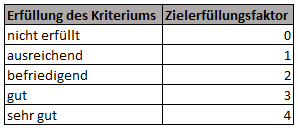
\includegraphics[width=1\textwidth]{gfx/Picture/Ziel.PNG}
 \caption{Die Zielerfüllungsfaktor-Tabelle mit einem Bereich von null bis vier}
 \label{fig:Ziel}
\end{figure}
\newpage
\begin{figure}[h!]
 \centering
 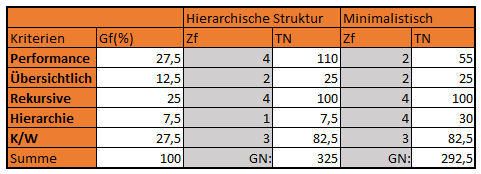
\includegraphics[width=1\textwidth]{gfx/Picture/Nutzwert.PNG}
 \caption{Nutzwertanalyse für die beiden Konzepte}
 \label{fig:Nutz}
\end{figure}

Wie in der Grafik (\ref{fig:Nutz}) erkennbar ist, ist der \ac{GN} zwischen den beiden Faktoren bei $70$.
Da der Unterschied zu klein ist, werden die Wertmaßstäbe weiter verfeinert.
Deswegen wird die \ac{Zf} verdoppelt, um einen eindeutigeren Unterschied zu erkennen.
Dadurch ändert sich die Punkteskala und die Tabelle wie folgt:
\begin{figure}[h!]
 \centering
 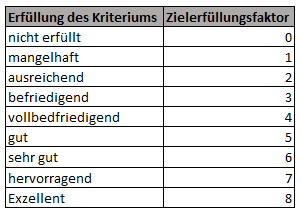
\includegraphics[width=1\textwidth]{gfx/Picture/Ziel2.PNG}
 \caption{Die erweiterte Zielerfüllungsfaktor-Tabelle von null bis acht}
 \label{fig:Ziel}
\end{figure}
\newpage
\begin{figure}[h!]
 \centering
 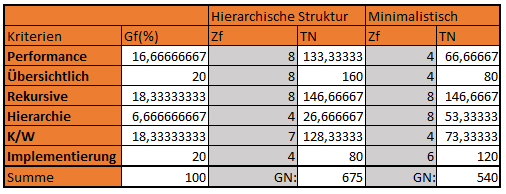
\includegraphics[width=1\textwidth]{gfx/Picture/Nutzwert2.PNG}
 \caption{Nutzwertanalyse für die beiden Konzepte}
 \label{fig:Nutz}
\end{figure}
Durch die Verfeinerung liegt der Unterschied zwischen den beiden Faktoren bei $135$, wodurch das Konzept der hierarchischen Struktur eindeutig der Rangfolge an der ersten Stelle steht.

\section{Vor/Nachteile der hierarchischen Struktur}
\label{sec:chapter05:Hierarchische}
Bei der ersten Tabelle (\ref{fig:Ziel}) wurden der hierarchischen Struktur für Performance vier, für Übersichtlichkeit vier, für Rekursion vier, für Hierarchie eins, für \ac{K/W} vier und für die Implementierung zwei Punkte gegeben.
Die Performance hat vier bekommen, da die Effizienz durch den Algorithmus im Allgemeinfall um die 50 Mal effektiver ist.
Dies ist eine enorme Steigerung, weshalb es die maximale Punktzahl bekommen hat.
Die Übersichtlichkeit hat vier Punkte erhalten, weil die Entwickler einstimmig dieses Konzept als übersichtlicher empfinden.
Zudem ist es einfacher festzustellen, welches Profil, welche Aufgabe hat.
Aber es hat zwei Punkte dadurch verloren, dass die Grafik bei weiteren Profilen schwieriger zu lesen wird, da diese größer ist.
Rekursion hat vier Punkte erlangt, da durch die Regelung, dass Profile nur noch Profile oder Berechtigungen enthalten sowie die feste Struktur keine rekursiven Beziehungen möglich sind, sofern diese Regelungen nicht aktive verletzt werden.
Deshalb hat es wie Performance vier Punkte erhalten.
Für die Hierarchie hat die Struktur nur einen Punkt bekommen, weil es bei diesem Punkt darum ging, die Hierarchie so stark wie möglich zu verringern.
Es ist besser als die vorherige Hierarchie, aber dennoch sehr hierarchisch.
Die \ac{K/W} haben nur vier Punkte bekommen, da nach der Entwicklung der Profile, diese nicht mehr geändert werden sollen.
Die Implementierung hat lediglich zwei Punkte bekommen, da diese aufwendig ist.
\newline
\newline
Nachdem die \ac{Zf} erweitert wurde, haben sich die Werte wie folgt verändert.
Der Performance wurden acht Punkte, der Übersichtlichkeit acht, der Rekursion acht, der Hierarchie vier, der \ac{K/W} sieben und der Implementierung vier Punkte gegeben.
Wie schon im vorherigen Absatz angegeben wurde, kann dieses Konzept 50 Mal effektiver sein.
Deshalb habe ich diesem Punkt exzellent gegeben, da dies eine deutliche Verbesserung ist.
Die Übersichtlichkeit hat ebenso eine exzellente Bewertung erhalten.
Die Struktur ist geordnet nach den Fachbereichen und hat ein Hierarchielimit von vier.
Dies ist der Rahmen, wodurch die IT-Spezialisten dies als übersichtlich befinden.
In der Kategorie Rekursion ändert sich nicht viel, weshalb es wieder volle Punktzahl erlangt.
Die Hierarchie hat vier Punkte bekommen, da die Hierarchie, wenn auch nur minimal, verringert wurde.
Dies würde nur drei Punkte geben, aber da auch die Hierarchiestufen auf vier limitiert wurden, hat dies einen weiteren Punkt gegeben.
\ac{K/W} hat nur sieben statt acht Punkte bekommen, da dieses Konzept, trotz dessen, dass es nicht geändert werden soll, in einem regelmäßigen Zyklus gewartet werden muss.
Dies liegt daran, dass man überprüfen muss, ob nicht ein Entwickler aus Faulheit die Struktur geändert hat.
Daher ist es eine hervorragende Lösung, aber dennoch müssen die o.g. Punkte berücksichtigt werden.
\newline
\newline
Zusammenfassend hat das Konzept der hierarchischen Struktur viele positive Aspekte, u.a. die erhöhte Performance sowie die Rekursion und die Übersichtlichkeit.
Auf der anderen Seite ist dieses Konzept weiterhin sehr hierarchisch und die Implementierung ist aufwendig.
Dies würde einiges an Personentagen sowie weiteres Geld kosten.

\section{Vor/Nachteile minimalistische Struktur}
\label{sec:chapter05:Minimalistisch}
Das Konzept der minimalistischen Struktur hat für die Performance zwei, die Übersichtlichkeit eins, die Rekursion vier, die Hierarchie vier, die \ac{K/W} zwei und die Implementierung vier Punkte erhalten.
Durch die verringerte Struktur hat sich die Performance ebenso verbessert, aber dies ist keine permanente Lösung, da ein Ansteigen der Profilanzahl diesen Bonus nichtig macht.
Aus diesem Grund hat es nur zwei Punkte bekommen.
Bei der Übersichtlichkeit hat nur einen Punkt erlangt.
Auch wenn durch das Entfernen der Hierarchie weniger Verwirrung herrscht, ist es dennoch sehr unübersichtlich, wenn alle Berechtigungen, mit Ausnahme der Standardberechtigungen, direkt am Profil hängen.
Da es keine tiefe Hierarchie mehr gibt, ist es auch unmöglich, dass es eine Rekursion gibt.
Deshalb erlangt dieses Konzept in diesem Punkt die maximale Anzahl von Punkten.
Wie schon angesprochen geht es bei dem Punkt Hierarchie darum, die Hierarchie so stark wie möglich zu reduzieren und dieses Konzept hat die Hierarchiestruktur auf ein Minimum gebracht. Somit erhält es vier Punkte.
Die \ac{K/W} haben zwei Punkte erlangt, da regelmäßig überprüft werden muss, ob Entwickler nicht aus verschiedenen Gründen zusätzliche Profile hinzufügen.
Dies ist eine Sorge, da genau dies zur unübersichtlichen Berechtigungsstruktur geführt hat, die die Helvetia aktuell hat.
\newline
\newline
Nach der Spezifizierung hat sich die Bewertung des minimalistischen Konzepts wie folgt geändert.
Die Performance wurde auf vier Punkte angepasst. Ebenso wurde die Übersichtlichkeit auf vier, die Rekursion auf acht, die Hierarchie auf acht, die \ac{K/W} auf vier und die Implementierung auf sechs Punkte geändert.
Der Punkt Performance hat die Bewertung befriedigend bekommen, da diese eine Verbesserung zur ursprünglichen Struktur ist.
Dennoch muss berücksichtigt werden, dass sich dies mit einer wachsenden Struktur verschlechtern wird, weshalb diese Verbesserung nur temporär ist.
Die Übersichtlichkeit hat die Note gut statt ein vollbefriedigend erhalten.
Auch wenn durch die Struktur die Beziehungen zwischen den Berechtigungen und dem Nutzer simpler sind, ist das Betrachten dieser schwierig, wenn die Anzahl der Berechtigungen wächst.
Dies liegt daran, dass die Berechtigungen nicht mehrmals an verschiedenen Stellen dem Profil zugewiesen werden.
Die Rekursion erlangt ein exzellent, da es nicht möglich ist, eine rekursive Beziehung zu erstellen, außer, wenn ein Standardprofil auf sich selber zeigt.
Die Hierarchie hat ebenso wie die Rekursion ein exzellent erhalten, da eine weitere Reduktion der Hierarchie für lediglich mehr Chaos sorgen würde, da dann alle Berechtigungen direkt am Nutzer hängen.
Die \ac{K/W} erlangt vier Punkte. 
Das minimalistische Konzept hat nicht viele Konventionen, die überprüft werden müssen.
Ebenso ist die Überprüfung einfach, da die Struktur so minimalistisch ist, aber regelmäßig überprüft werden muss und das Risiko, dass ein Entwickler die Struktur ändert, ist hoch.
\newline
\newline
Zusammenfassend kann gesagt werden, dass das minimalistische Konzept am hilfsreichsten ist, wenn man nach spezifischen Berechtigungen sucht.
Durch die minimale Hierarchie gibt es nicht viele Stellen, die überprüft werden müssen oder Stellen, an denen Rekursionen entstehen können.
Auf der anderen Seite ist jedoch die Verbesserung der Performance nicht stabil und kann sich schnell ändern, wenn weitere Profile hinzugefügt werden.
Die Implementierung ist im Verhältnis zum Konzept der hierarchischen Struktur deutlich einfacher, da für jeden Fachbereich die Standardprofile entwickelt werden müssen und ansonsten die restlichen Berechtigungen direkt den Nutzern zu geteilt werden. Dadurch müssen keine neuen Profile entwickelt werden.
Jedoch besteht die Gefahr, dass bei der Menge von Berechtigungen gewisse Nutzer bestehende Berechtigungen verlieren.
Zudem könnte die Anzahl der individuellen Berechtigungen ein Problem darstellen, wenn diese abgespeichert werden sollen.

\section{Ablösung durch RACF}
\label{sec:chapter05:racF}
Neben dem aktuellen DB$2$ Tabellen Modell ist auch intern der Gedanke aufgekommen, dass die bestehende Struktur in das \ac{RACF} ausgelagert werden kann.
Den die Helvetia verwendet aktuell schon \ac{CICS} von IBM für die Kommunikation der internen Prozesse.
Dabei wird auch das \ac{RACF} verwendet.
Aus diesem Grund wurde überlegt, ob nicht die DB$2$ Tabellen ebenso in diese Umgebung integriert werden sollen.
Das hätte den Vorteil, dass sämtliche Prozesse an einem Ort stattfinden und daher die Suche etwas vereinfacht ist.
Zudem wäre dies ein Schritt, um sich von der Welt des Hosts weiter zu distanzieren.
Dies wäre ein positiver Aspekt, wenn das Unternehmen sich in der Zukunft vom Host lösen möchte.
\newline
\newline
Für den Wechsel von der DB$2$-Tabelle zu \ac{RACF} würden die Profile, Nutzer und Berechtigungen wie folgt geändert werden:
\begin{itemize}
	\item Die HDM-Vorgangsprofile werden mittels Data Control Groups dargestellt
	\item Die Berechtigungen werden durch General Resource Profiles abgebildet
	\item Die Nutzer werden anhand von Holding Groups verkörpert
\end{itemize}
Die Data Control Groups fungieren als ein Schnittpunkt für die Daten, welche vor nicht autorisierten Zugriff geschützt werden sollen. \cite{IBMdcg}
Die General Ressource Profiles bieten einen Schutz an für Computer Ressourcen sowie andere Datenformate wie zum Beispiel Berechtigungen. \cite{IBMgrp}
Die Nutzer werden als Holding Group dargestellt, da diese den Nutzer in das bestehende System integriert, dieser aber kaum Berechtigungen erhält, wodurch er keinen Zugriff auf die Berechtigungen hat.
Dies muss über einen Administrator, welcher über die CONNECT Autorität verfügt, verwaltet werden, damit der Nutzer seine Berechtigungen erhält. \cite{IBMhg}
\newline
\newline
Auf der anderen Seite bestehen jedoch die folgenden Probleme:
\begin{itemize}
	\item Bestehende Schnittstellen
	\item Transfer der Daten
	\item Schulung des Personals
\end{itemize}
Die aktuelle DB$2$-Tabelle verfügt über verschiedene Schnittstellen für die Abfrage von Berechtigungen.
Wenn diese durch das \ac{RACF} ersetzt werden sollen, müssen diese durch neue Schnittstellen ersetzt werden.
Im Gespräch mit den IT-Spezialisten wurde gesagt, dass dies ein großes Problem darstellt, da dafür eine spezielle Application Programming Interface entwickelt werden müsste.
Dies würde neben dem normalen Wechsel von den DB$2$-Tabellen zu \ac{RACF} für weitere Kosten sorgen.
\newline
Ein anderes Problem ist auch der Transfer der bestehenden Daten in das \ac{RACF}.
Für diesen Prozess müsste auch hier eine Schnittstelle entwickelt werden, welche bei dem Transfer die Daten in das richtige Dateiformat transformiert.
Neben den steigenden Kosten besteht auch das Risiko, dass bei der Transformation ein Fehler geschieht.
\newline
Selbst wenn die vorherigen beiden Punkte kein Problem darstellen, muss dennoch das gesamte Personal, welches mit den Tabellen gearbeitet hat, für das \ac{RACF} geschult werden.
Dies würde weitere Personentage kosten.
Aufgrund dieser Faktoren ist der Wechsel in das \ac{RACF} nicht ratsam, da zu viele große Probleme bestehen, welche Geld und Zeit kosten werden.
\newline
Sollte Helvetia sich dennoch für das \ac{RACF} enscheiden, würde der Algorithmus wie in der Grafik (\ref{fig:racf}) aussehen:
\begin{figure}[h!]
 \centering
 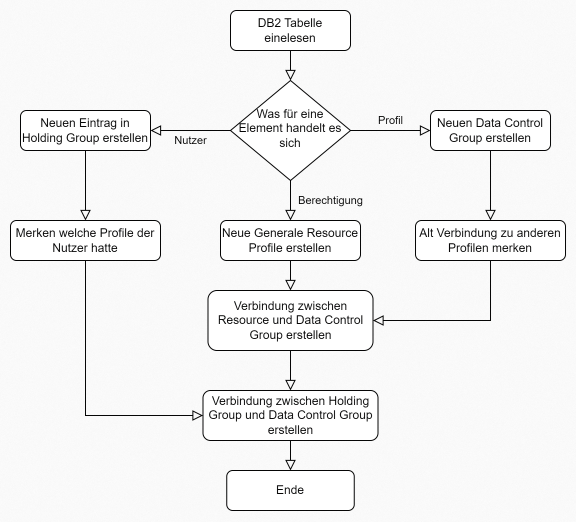
\includegraphics[width=1\textwidth]{gfx/Picture/racf.PNG}
 \caption{Algorithmus für den Wechsel zu RACF}
 \label{fig:racf}
\end{figure}